\documentclass[a4paper]{article}
\usepackage[cmex10]{amsmath}
\usepackage{amssymb}
\usepackage{amsthm}
\usepackage{array}
\usepackage{bm}
\usepackage{graphicx}
\usepackage{epstopdf}
\usepackage[hang]{subfigure}
\usepackage{import}
\usepackage{booktabs}
\usepackage{tabularx}

\usepackage[colorlinks=true,linkcolor=blue,citecolor=blue,urlcolor=black]{hyperref}
\usepackage{algorithm, algpseudocode}

\usepackage[nottoc]{tocbibind}

% Commenting functionality
\usepackage{todonotes}
%\reversemarginpar

\usepackage{pifont}
\newcommand{\cmark}{\ding{51}}%
\newcommand{\xmark}{\ding{55}}%

\newcommand{\brs}[1]{\left[{#1}\right]} %square bracets
\newcommand{\brr}[1]{{\left({#1}\right)}} %round bracets
\newcommand{\brf}[1]{\left\lbrace{#1}\right\rbrace} %figure bracets
\newcommand{\brabs}[1]{\left\vert{#1}\right\vert} %absolute bracets
\newcommand{\norm}[2]{\left\|{#1}\right\|_{#2}} %norm_*

\newcommand{\I}[1]{\ensuremath{I\!\left[{#1}\right]}} %Robustness criterion I[*]
\newcommand{\Iq}[1]{\ensuremath{I_q\!\left[{#1}\right]}} %Robustness criterion I_q[*]
\newcommand{\Ic}[1]{\ensuremath{I_c\!\left[{#1}\right]}} %Robustness criterion I_c[*]

\newcommand{\vx}{\ensuremath{\mathbf{x}}} % vector x
\newcommand{\vX}{\ensuremath{\mathbf{X}}} % vector X
\newcommand{\vf}{\ensuremath{\mathbf{f}}} % vector f
\newcommand{\vz}{\ensuremath{\mathbf{z}}} % vector z
\newcommand{\vZ}{\ensuremath{\mathbf{Z}}} % vector Z
\newcommand{\vw}{\ensuremath{\mathbf{w}}} % vector w
\newcommand{\vd}{\ensuremath{\mathbf{d}}} % vector d
\newcommand{\vp}{\ensuremath{\mathbf{p}}} % vector p
\newcommand{\vP}{\ensuremath{\mathbf{P}}} % vector P
\newcommand{\vu}{\ensuremath{\mathbf{u}}} % vector u
\newcommand{\vU}{\ensuremath{\mathbf{U}}} % vector U
\newcommand{\DSet}{\ensuremath{\mathcal{D}}} % Set D
\newcommand{\NSet}{\ensuremath{\mathcal{N}}} % Set N
\newcommand{\XSet}{\ensuremath{\mathcal{X}}} % set X
\newcommand{\ZSet}{\ensuremath{\mathcal{Z}}} % set Z
\newcommand{\SSet}{\ensuremath{\mathcal{S}}} % set S
\newcommand{\Pref}{\ensuremath{\mathcal{P}}} % Preferences set P

\DeclareMathOperator*{\argmin}{\arg\!\min}
\DeclareMathOperator*{\argmax}{\arg\!\max}


\begin{document}
\title{WP1 M4 -- Methodology for a robust design optimization framework}
\date{\today, v1.0}
\maketitle

\setcounter{tocdepth}{3}
\tableofcontents

\section{Introduction}
\subsection{Context}
The framework for robust design optimization, developed under PSi T8 WP1, is aimed at design activities involving multiple objectives and featuring uncertainties of various sources. The framework intends to support the goal of a ``right-first-time-design", where appropriate design choices are made based on computer simulations alone. In this context, a high quality solution does not necessarily have to demonstrate the very best possible performance under a single set of assumptions, but rather to perform well under a large variety of uncertain factors. The requirements for the framework were previously identified in milestone report WP1 M3. The current report, WP1 M4, describes the methods adopted and developed by the Theme 8 research team to deliver the ``must have'' requirements identified at M3.

\subsection{Background}
The ability of numerical simulations to predict the performance of a candidate design is constantly increasing. While some simulations can produce high-fidelity outputs relatively quickly, a typical mesh-based simulation can run for several hours, and even days. Even if a design team has access to supercomputing resources, the extensive run-time still implies that perhaps only a few hundred candidate designs can be explored using high-fidelity modelling resources. Unfortunately, conventional multi-objective optimization algorithms, such as NSGA-II \cite{deb2002fast}, implemented in commercial packages typically require tens of thousands of function evaluations to converge on a high quality solution~\cite{Hansen2010Comparing,Zhou2011Multiobjective}. Therefore, the search for a promising design using expensive evaluation functions on a limited computational budget poses a great challenge.

To exacerbate this problem, optimizing for a \emph{robust} solution is itself a computationally demanding task. In order to gain confidence over the robustness of a solution to uncertainties, the statistical properties of the expected solution's performance must be quantified. In a world where the complexity of the high-fidelity models essentially produces a black-box mapping of inputs to outputs, such statistical properties would typically be found through repeated evaluation of the same solution using those high-fidelity models. Such Monte Carlo sampling of a single candidate design is computationally expensive.

The framework we have developed aims to address these challenges for a single optimization node, situated within a wider family of nodes simultaneously working on the design of a complex engineered product. From the single-node perspective, the key characteristics of the problem formulation can be summarised as follows:
\begin{itemize}
	\item Expensive, black-box evaluation functions for a candidate design
	\item Many objectives to be addressed simultaneously (i.e.~more than three)
	\item Multiple sources of uncertainty:
	\begin{itemize}
		\item Fidelity of evaluation functions
		\item Manufacturing tolerances
		\item Inherent variation of operating conditions
		\item Uncertainty over the state of shared or coupled design choices
	\end{itemize}
	\item Interaction with a designer or decision facilitator:
	\begin{itemize}
		\item Working with robustness metrics to provide an understanding of the risk and opportunity trade-offs between candidate designs
		\item Working with user preferences to steer the search towards a desirable compromise solution.
	\end{itemize}
\end{itemize}

\subsection{Relevant literature}
The framework leverages ParEGO~\cite{knowles2005multiobjective,Knowles2006ParEGO}, an algorithm for multi-objective optimization, which has been demonstrated to provide good results for optimization runs limited to a small number of function evaluations. ParEGO itself is a multi-objective extension to Jones et al.'s~\cite{Jones1998Efficient} seminal \emph{efficient global optimization} (EGO) algorithm for single-objective problems.

EGO is designed to search for the global optimum of a single, computationally expensive objective function. It uses a surrogate model estimated from previously evaluated designs to guide the search. An iterative procedure is performed to evaluate the design that has the highest probability to improve both the expected performance and the model's accuracy. The structure of EGO is as follows: first, an initial set of candidate solutions is constructed using Latin hypercube sampling~\cite{Scheffe1958Experiments}, and evaluated by the expensive evaluation function. Next, the following iterative procedure is repeated: the existing evaluations are considered as an outcome of a stochastic process, and are used to construct a so-called \emph{design and analysis of computer experiments} (DACE) model~\cite{Sacks1989Design}, which maximizes the likelihood of the fitted model to the basis (i.e.~known) points. The advantage of the DACE model is that it provides an estimation of its own error, in addition to the estimated function value at every point. \footnote{For further details on the DACE model, please refer to the original paper \emph{Design and Analysis of Computer Experiments}~\cite{Sacks1989Design} and the excellent summary in~\cite{Jones1998Efficient}.}

Figure~\ref{fig:EGO} depicts a univariate DACE model fitted to five evaluated points. The model prediction and its error are shown in blue and red lines, respectively. Since the choice of model is constrained such that its output is identical to that of the evaluated points, the error at these points is zero. The function value over the rest of the space is considered as a normally-distributed random variable with mean and standard error given by the DACE model and its error, respectively: $F\brr{\vx}\sim N\brr{\hat{f}\brr{\vx},\hat{\sigma}^2\brr{\vx}}$.
\begin{figure}
	\centering
	\def\svgwidth{\textwidth}
	\import{figures/}{EGO.pdf_tex}
	\caption{Interpolation of the evaluated points (black) with a DACE model (blue). Estimation error is shown in red (not in scale). The uncertainty about the function value is considered as a normal distribution with mean and standard error according to the DACE model at every point.}
	\label{fig:EGO}
\end{figure}

Once the model is constructed, a search is conducted to locate the design that has the highest probability of improving the objective value over the currently best design, denoted as $f_\text{min}$. For minimization, the improvement at point $\vx$ is $Q\brr{\vx}=\max\brr{f_\text{min}-F\brr{\vx},0}$. The expected improvement $E\brs{Q\brr{\vx}}$ has a closed form expression~\cite{Jones1998Efficient}:
\begin{align}
E\brs{Q\brr{\vx}} = \brr{f_\text{min}-\hat{f}}\Phi\brr{\frac{f_\text{min}-\hat{f}}{\hat{\sigma}}} + \hat{\sigma}\phi\brr{\frac{f_\text{min}-\hat{f}}{\hat{\sigma}}},
\end{align}
where $\Phi\brr{\cdot}$ and $\phi\brr{\cdot}$  are the standard normal distribution and density functions, respectively, and $\hat{f}$ and $\hat{\sigma}$ are short-hand notations for $\hat{f}\brr{\vx}$ and $\hat{\sigma}\brr{\vx}$.

By maximizing the expected improvement, exploration and exploitation of the global search are automatically balanced. This is because unexplored regions have larger prediction error, and therefore they might have larger probability for improvement than explored regions, even if the expected value is higher. The procedure is terminated when no solution is found that is expected to improve the current best value, or when the budget of function evaluations has been reached.

The following assumptions are made by the EGO algorithm:
\begin{enumerate}
	\item Expensive evaluation function --- this justifies the amount of computation effort expended between consecutive function evaluations.
	\item Black-box evaluation function --- no other information is know on the function and its derivatives that can support estimation of the function without full evaluation.
	\item Deterministic problem --- uncertainties are not present in any part of the problem formulation, and therefore repeated evaluations of the same design yield the same result.
	\item Single objective problem --- multi-objective optimization is not considered.
	\item Locally smooth and continuous evaluation function --- the DACE model assumes spatial correlation in decision-space.
This means that close solutions are expected to have similar function values.
	\item Low-to-medium number of decision variables --- the DACE model's accuracy reduces when the dimensionality of the decision-space exceeds approximately 20 variables~\cite{Knowles2006ParEGO}.
\end{enumerate}

Knowles~\cite{Knowles2006ParEGO} extended EGO to solve multiobjective optimization problems with his algorithm ParEGO (the name implies the search for Pareto optimality). Apart from Assumption 4, ParEGO addresses the same types of problems as EGO. To achieve a multi-objective formulation, the overall multi-objective problem is decomposed into a number of single-objective problems by using a set of weighting vectors and a scalarising function (known as the weighted Chebyshev). More details on decomposition strategies are provided in Section~\ref{sec:Decomposition}. For every iteration of the optimizer, a random weighting vector is drawn from the available set, and a DACE model is constructed from the scalarised values of each objective vector. The next candidate solution to be investigated is the one with the highest expected improvement of the scalar function using the current weighting vector.

The effectiveness of ParEGO at performing multi-objective optimization on a limited budget of function evaluations makes it a key candidate for further development for the purposes of the framework. There has been substantial progress in the literature on decomposition-based algorithms since ParEGO was published in 2005 (see~\cite{Giagkiozis2013Overview} and references within) suggesting the potential for further improvements in performance. The main limitation of ParEGO is that it has not been designed to handle problems featuring uncertainty (although there is some evidence that it can perform favourably in noisy environments \cite{knowles2009noisy}). Therefore a fundamental part of the framework is how ParEGO can be extended to consider evaluation functions as samples of random variates. We refer to this new algorithm as \emph{stochastic ParEGO} or \emph{sParEGO}.

\subsection{Overview}
In Section~\ref{sec:Decomposition} the decomposition-based approach to multi-objective optimization, which forms the heart of the framework, is introduced. In Section~\ref{sec:Uncertainty Approximation}, the innovations to enable an effective search under uncertainty are developed in detail. Section~\ref{sec:Robustness Indicators} introduces the  metrics that are used to operationalise the notion of robustness and Section~\ref{sec:sParEGO} summarises the complete sParEGO algorithm. Section~\ref{sec:Other aspects} provides a brief account of the remaining aspects of the framework needed to deliver the ``must have'' requirements from WP1 M3, and the report concludes in Section~\ref{sec:conclusion} with a roadmap for the remainder of WP1.

For convenience, the notation used throughout the report is summarised in Table~\ref{tab:Nomenclature}.

\begin{table}
\caption{Nomenclature}
\begin{tabular}{p{1.5cm}cp{2.5cm}cp{1.5cm}cp{3.5cm}} \toprule
{\bf Notation}	&& {\bf Meaning}					&& {\bf Example}				&& {\bf Description}											\\ \midrule
Lower case		&& scalar variable					&& $x$							&& a deterministic decision variable or a realisation of a random decision variable\\ \midrule
Upper case		&& random variable					&& $X$							&& a random decision variable $X$ that follows a certain distribution \\ \midrule
Bold face		&& vector							&& $\vx$						&& vector of decision variables									\\ \midrule
Square brackets && vector							&& $\brs{v_1,v_2,v_3}$			&& vector $\bm{v}$ with three components						\\
				&& indicator						&& $\I{S}$						&& a scalar value to evaluate the robustness of the random variable $S$	\\ \midrule
Subscript		&& component of a vector			&& $x_i$						&& $i^\text{th}$ decision variable								\\
				&& property of a random variable	&& $\mu_s$						&& mean value of random variable $S$							\\ \midrule
Calligraphic	&& set								&& $\XSet$						&& set of decision vectors										\\ \midrule
Curly brackets  && set								&& $\brf{\vz^1,\ldots,\vz^n}$	&& set $\ZSet$ with $n$ vectors									\\ \midrule
Superscript		&& member of a set					&& $\vx^j$						&& $j^\text{th}$ decision vector								\\
				&& 									&& $x^j_i$						&& $i^\text{th}$ variable of the $j^\text{th}$ decision vector	\\ 
\bottomrule
\end{tabular}
\label{tab:Nomenclature}
\end{table}

\section{A decomposition-based approach to multiobjective optimization}
\label{sec:Decomposition}
A multiobjective optimization problem (MOP) can be described as:
\begin{align}
\label{eq:mop}
	\min_{\vx\in\Omega} \vz=\vf\brr{\vx},
\end{align}
where \vx\ is a vector of $n_x$ decision variables in a feasible domain $\Omega$, \vz\ is a vector of $n_z$ performance criteria and \vf\ is a set of functions mapping from decision-space to objective-space:
\begin{align}
	\vf: \mathbb{R}^{n_x} \rightarrow \mathbb{R}^{n_z}
\end{align}
If some of the objectives are in conflict with one another, the solution to~\eqref{eq:mop} is expected to be a set of decision vectors, offering different trade-offs between the objectives.

\subsection{Normalisation} 
\label{subsec:Normalisation}
The decision variables and objectives are likely to be incommensurable, and therefore both decision-space and objective-space are normalised to non-dimensional units in the following manner:

\begin{align}
	\tilde{x}_i &= \frac{x_i - x^l_i}{x^u_i - x^l_i} , &i=1,\ldots,n_x,\\
	\tilde{z}_j &= \frac{z_j - z^*_j}{z^n_j - z^*_j} , &j=1,\ldots,n_z,
\end{align}
where $x^u_i$ and $x^l_i$ are the upper and lower boundaries of the $i^\text{th}$ decision variable, $z^n_j$ and $z^*_j$ are the $j^\text{th}$ components of the known nadir and ideal vectors\footnote{The ideal vector is composed of the best value of each objective. The nadir vector is composed of the worst value of each objective amongst all Pareto optimal solutions. Both vectors are estimated according to the current available information concerning the objective-space.}, and the tilde accent represents a normalised, dimensionless variable.

The normalised values are used for all operations within the algorithm. Before a candidate design is evaluated, it is re-scaled to the natural dimensions.

\subsection{Scalarising functions}
\label{subsec:Scalarising}
Over the last decade, decomposition-based evolutionary methods have gained increasing popularity for solving multiobjective optimization problems~\cite{Giagkiozis2013Overview}. A decomposition-based algorithm decomposes the MOP~\eqref{eq:mop} into $n$ single-objective problems, each targeting different ratios between the objectives. This sort of decomposition can be seen in Figure~\ref{fig:decomposition}: a set of six reference objective vectors is being used to guide the search towards different regions on the Pareto front. A different sub-problem is defined for every direction vector by using a scalarising function $f\brr{\vz,\vw}$ that maps an objective vector \vz\ into a scalar value according to a vector of weights \vw. The weights vector \vw\ is composed of non-negative components that sum to one.
The $i^\text{th}$ component of \vw\ is the relative weight of objective $z_i$.

\begin{figure}
	\centering
	\def\svgwidth{0.4\textwidth}
	\import{figures/}{decomposition.pdf_tex}
	\caption{Decompostion of a bi-objective problem into six single-objective problems, each aiming at a different ratio between the objectives.
	Reference direction vectors are marked in grey and corresponding Pareto optimal solutions in black.}
	\label{fig:decomposition}
\end{figure}

The scalarising function used in this framework is the popular \emph{weighted $L_p$}~\cite{koski1987norm,Marler2004Survey}:
\begin{align}
\label{eq:weighted Lp}
	s = \brr{\sum_{i=1}^{n_z} \brr{w_i\cdot \brr{z_i-z_i^*}}^p}^{1/p},
\end{align}
where $\mathbf{z^*}$ is a reference vector in objective space, typically the \emph{ideal} vector, which is composed of the minima of each individual objective. For a given weighting vector $\vw$, a comparison between two vectors $\vz^{A}$ and $\vz^{B}$ depends on the choice of norm $p$. Figure~\ref{fig:weightedLp} depicts the effect of using different values of $p$ for a bi-objective problem. The black point represent a desired ratio between the two objectives $\brs{0.3,0.7}$, and the black line passing through this point denotes all the objective vectors with this ratio. The coloured lines represent contours of the scalarising function of Equation~\eqref{eq:weighted Lp}. It can be seen that as the norm increases, vectors closer to the black direction line have lower function values than other non-dominated vectors farther away from the line.
\begin{figure}% 3D graphical demonstration
\centering
\subfigure[$p=1$]{
\label{subfig:weightedLp p1}
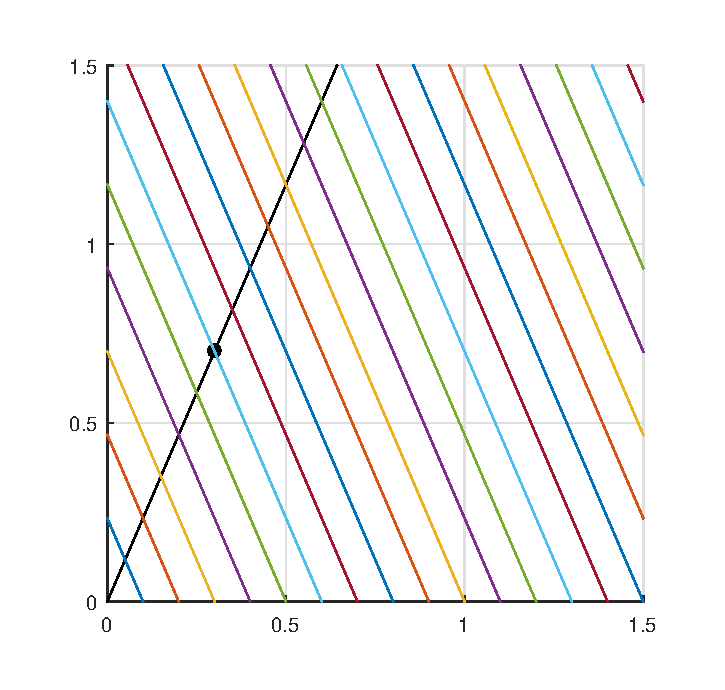
\includegraphics[width=0.31\textwidth]{figures/projectionContoursP1.eps}}
\subfigure[$p=3$]{
\label{subfig:weightedLp p3}
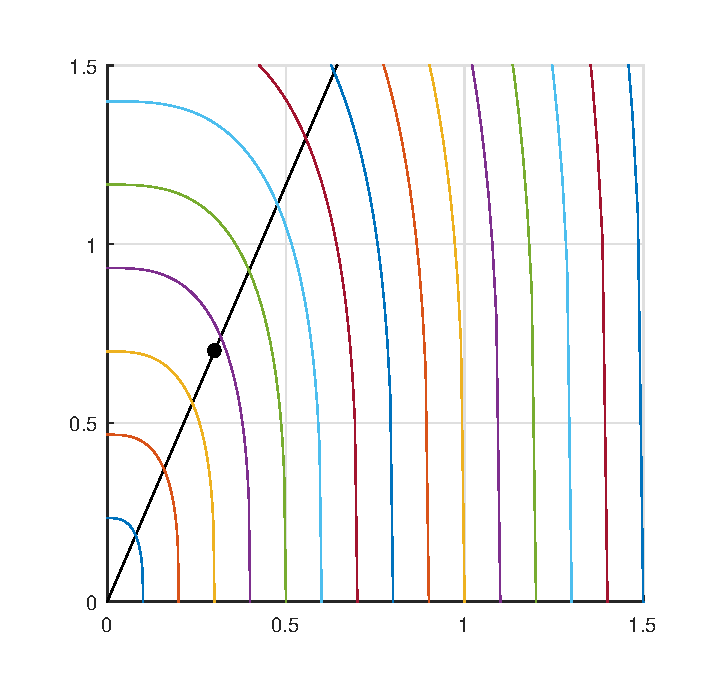
\includegraphics[width=0.31\textwidth]{figures/projectionContoursP3.eps}}
\subfigure[$p=50$]{
\label{subfig:weightedLp p50}
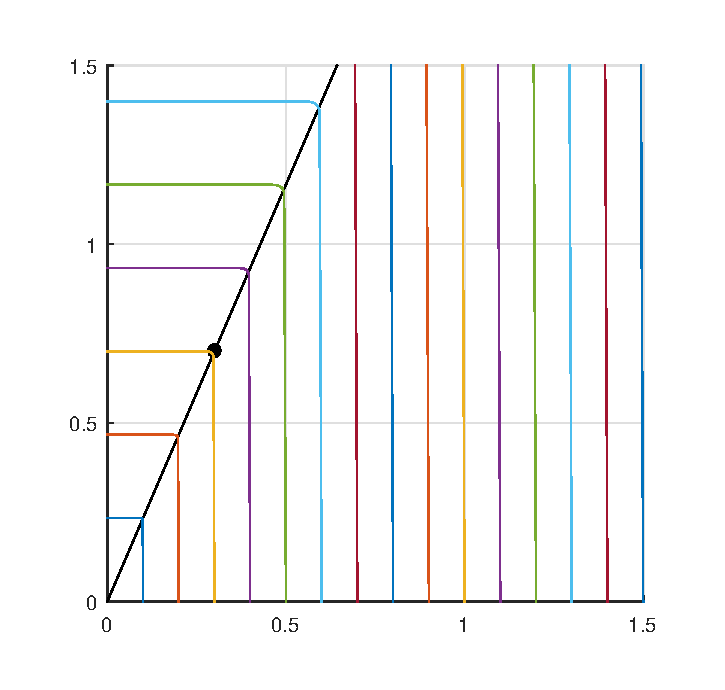
\includegraphics[width=0.31\textwidth]{figures/projectionContoursP50.eps}}
\caption{Contours of equal function values~\eqref{eq:weighted Lp} for different norms $p$}
\label{fig:weightedLp}
%% label for entire figure
\end{figure}

A high value of $p$ guarantees that the Pareto optimal solution that minimizes the scalarising function will possess the desired ratio between objectives. However, by using a higher norm the convergence of the algorithm becomes slower, since the focus is given to the single objective that has the largest deviation from the reference vector (as perhaps first noted in the literature in~\cite{borges1998basis}). In sParEGO, the weighted sum ($p=1$) is used in early stages to promote convergence, and the norm is gradually increased towards the final stages of the algorithm in an effort to find a well distributed set of solutions to present as possible trade-off choices.

For a given direction vector \vd\ there is a corresponding weighting vector that minimizes the scalarising function \cite{giagkiozis2014generalized}. The optimal weighting vector $\mathbf{w}$ for the scalarising function in~\eqref{eq:weighted Lp} is defined as:
\begin{align}
\begin{split}
	&\mathbf{w}=\brs{w_1,\ldots,w_{n_z}},\\
	&w_i=a\cdot\brr{d_i+\epsilon}^{-1} \quad , \quad i=1,\ldots,n_z,\\
	&\sum_{i=1}^{n_z} w_i=1,
\end{split}
\end{align}
where $\epsilon$ is a small number to prevent division by zero, and $a$ is a normalisation factor.

\subsection{Preference elicitation}
\label{subsec:preference}
To focus the search towards desired solutions, the framework allows a decision facilitator to indicate which regions of objective-space are of interest. The flexible method suggested by Wang et al.~\cite{Wang2013Whatever} is adopted to identify a limited set of direction vectors in objective-space, according to the user's specifications. The preferences can be specified before the search begins by setting goal vectors, or progressively, by interactively ``brushing'' interesting solutions as the search evolves.

\subsection{Set of reference direction vectors}
\label{sec:Simplex Lattice}
The multiobjective optimization problem is decomposed to $n$ sub-problems as described in Section~\ref{subsec:Scalarising}. Each sub-problem $i$ correspond to a reference direction vector $\vd_i$ from a set $\DSet$. In the case where no preference information exists, the set is constructed using a Simplex Lattice design~\cite{Scheffe1958Experiments}:
\begin{align}
	\label{eq:SimplexLattice}
	\begin{split}
		\DSet = \Biggl\lbrace\vd=\brs{d_1,\ldots,d_{n_z}}\quad \vert \quad &\sum_{j=1}^{n_z} d_j = 1 \quad \wedge \\
		& \forall j, \quad d_j = \frac{l}{h}, l\in\brf{0,\ldots,h} \Biggr\rbrace.
	\end{split}
\end{align}
The number of direction vectors is determined by the dimensionality of the objective space, and the constant $h$: $\vert\DSet\vert = \binom{h+n_z-1}{n_z-1}$. The direction vectors are evenly distributed along the hyperplane $\sum z_j = 1$.

If a set of preferences $\Pref$ has been identified (using the method described in Section~\ref{subsec:preference}), $\DSet$ is constructed according to the procedure in Algorithm~\ref{alg:SimplexLattice}.
\begin{algorithm}
\caption{\textsc{SimplexLattice($n_{max}$,\Pref)}}
\label{alg:SimplexLattice}
\begin{algorithmic}[1]
	\State $h \leftarrow 0$
	\State $\DSet' \leftarrow \emptyset$
	\While{$\brabs{\DSet'}<n_{max}$}
		\State $\DSet \leftarrow \DSet'$
		\State $h \leftarrow h+1$
		\State generate $\DSet'$ according to Equation~\eqref{eq:SimplexLattice}
		\State remove all vectors $\vd\in\DSet'$ that do not satisfy all preferences $\Pref$
	\EndWhile
	\State \Return $\DSet$ after shuffling 
\end{algorithmic}
\end{algorithm}

\subsection{Constraint handling}
\label{subsec:constraints}
The feasible domain $\Omega$ in Equation~\eqref{eq:mop} can be defined by a set of equality and inequality equations. We make a distinction between three types of constraints: box constraints~\eqref{eq:box}, inequality constraints~\eqref{eq:inequality} and equality constraints~\eqref{eq:equality}.
\begin{align}
\label{eq:box} &x_i^\text{lb} \leq x_i \leq x_i^\text{ub},& i&=1,\ldots,n_x,\\
\label{eq:inequality} &g_j\brr{\vx} \leq 0,& j&=1,\ldots,J,\\
\label{eq:equality} &h_k\brr{\vx} = 0,& k&=1,\ldots,K,
\end{align}
where $g_j\brr{\vx}$ and $h_k\brr{\vx}$ can be either linear or non-linear functions. The total number of constraint functions is denoted as $n_c=J+K$.

The box constraints are met by ensuring every decision variable is within the feasible interval upon creation and after every variation operator. The functional constraints, which may be evaluated by black-box evaluation functions in a similar fashion as the objectives, are handled by using a penalty method.

Penalty methods are the most common approach for handling constraints in evolutionary algorithms. The idea is to transform a constrained optimization problem to unconstrained by adding a penalty to the objective function based on the degree of constraint violation. By keeping infeasible solution instead of immediately rejecting them, valuable information can be used to steer the search towards feasible and optimal regions. For example, a solution with very good performance which slightly violates the constraints might be more useful than a feasible solution with very poor performance. A penalty function is described as:
\begin{align}
s^*\brr{\vx} = s\brr{\vx} + \brs{\sum_{j=1}^J w_{g,j}G_j\brr{\vx} + \sum_{k=1}^K w_{h,k}H_k\brr{\vx} }, 
\end{align}
where $s$ is the scalar objective function from~\eqref{eq:weighted Lp}, $G_j$ and $H_k$ are functions of the constraints $g_j$ and $h_k$, respectively, $w_{g,j}$ and $w_{h,k}$ are positive constants known as \emph{penalty factors}, and $s^*$ is the penalised objective function due to constraints violation. The choice of penalty function and the setting of the penalty factors has a substantial effect on the performance of the algorithm.

We adopt Farmani and Wright's method of \emph{self adaptive fitness formulation}~\cite{Farmani2003Self} for setting the penalty function. Its main advantage is that it automatically regulates the penalty factors and no parameter setting is required (see also~\cite{eiben1998adaptive} for excellent results from a similar method).

\section{Handling uncertainties}
\label{sec:Uncertainty Approximation}
The most important difference between sParEGO and ParEGO is that the former assumes that the outcome of an evaluation function is a realization of a random variate. Therefore, the scalarised function value cannot be used directly to construct the DACE model, and a utility indicator value is used instead. For every direction vector $\vd$, the surrogate model is constructed to search for a design that will optimize a given robustness indicator (described later in Section~\ref{sec:Robustness Indicators}). The guiding principle is to avoid Monte Carlo methods that repeatedly sample every candidate design to assess its statistical properties in objective-space. Instead, these properties (specifically, measures of central tendency and dispersion) are approximated from the available information of other candidate design evaluations.

The different sources of uncertainty, and the way they are propagated are described in Section~\ref{subsec:Uncertainty propagation}.
The steps for approximating the robustness indicator values of a set of candidate solutions are described in Section~\ref{subsec:Uncertainty quantification}. 

\subsection{Sources of uncertainty}
\label{subsec:Uncertainty propagation}
The framework allows for various sources of uncertainty, such as production variations, changing environmental conditions and model-method combination errors. 

\subsubsection{Working with uncertain inputs}
\label{subsubsec:uncertain inputs}
The method assumes that every uncertainty in the input space (either tolerances in the design or changes in environmental parameters) can be described by a probability function. When evaluating a design with its inherent uncertainties, $\vX$, under uncertain operating conditions, $\vP$, all uncertainty factors for both $\vX$ and $\vP$ are sampled from their distributions, and the sampled values are processed by the evaluation functions. The outcome of such evaluation, for each realisation of the uncertainty, is a single performance (or constraint) vector $\vz$. The left side of Figure~\ref{fig:uncertainties sampling} illustrates this procedure.

\begin{figure}  
	\centering
	\def\svgwidth{\textwidth}
	{\footnotesize 
	\import{figures/}{Uncertainties_sources.pdf_tex}
	}
	\caption{Handling different sources of uncertainties to evaluate a single sample of the performance vector. Random variables are marked with larger arrows.}
	\label{fig:uncertainties sampling}
\end{figure}

\subsubsection{Accounting for model uncertainties}
\label{subsec:model fidelity}
When models are used to simulate a physical phenomena, prediction errors are likely to occur. In this robust optimization framework, the model error adds another layer of uncertainty to those discussed in the previous section. To accommodate this uncertainty, a domain expert should specify the uncertainty of a simulation outcome $z$ as a random variable $Z$. For every model evaluation, instead of using the raw evaluation $z$, a sample $z'$ from the distribution $Z$ is used. This is illustrated in the right side of Figure~\ref{fig:uncertainties sampling}.

\subsubsection{Uncertainty associated with shared decision variables}
\label{subsec:Shared Decision Variables}
Nodes that feature shared decision variables are likely to be encountered in asynchronous distributed optimization problems. When two nodes are in conflict over the value of a shared decision variable, the framework offers a strategy to guide the search towards a compromise solution, acceptable to both nodes. A shared decision variable is considered to be a random variable $X$ with a mean value $\mu_x$ and variance $\sigma^2_x$. $\mu_x$ and $\sigma^2_x$ are approximated from the current choices of the other node(s) and the choice of the local node.

Assuming the other node's latest choices for $X$ is the set\footnote{Commonly in multiobjective optimization, a set of decision vectors is maintained, with possibly different values for the variable $X$.} $\chi^o=\brf{x^{o,1}, x^{o,2},\ldots,x^{o,n}}$. The average value of this set is:
\begin{align}
	\bar{x}^o &= \frac{1}{n}\sum_{i=1}^n x^{o,i}.
\end{align}
Given $\bar{x}^o$ and a local choice of $x$, the statistical properties of $X$ are:
\begin{align}
	\mu_x &= w^o \bar{x}^o + w^l x,\\
	\sigma^2_x &= \frac{w^o}{n}\sum_{i=1}^n \brr{x^{o,i}-\mu_x}^2 + w^l\brr{x-\mu_x}^2,
\end{align}
where $w^o$ and $w^l$ are the weights of decision of the other and local node, respectively. This weights are determined according to the influence of each node on the overall design process. A truncated normal distribution is fitted to the variable $X$ based on $\mu_x$ and $\sigma^2_x$, and the variable's boundaries.

This mechanism automatically resolves conflicts between the nodes: large variance degrades the performance of the solution, therefore a value closer to the other node's mean value is likely to be preferred, as long as it does not degrade the local node's objective too much. If node $A$ is more sensitive to variable $X$ than node $B$, the choices for this variable will tend to converge towards the value required by node $A$. The reason for this is that node $A$ will choose the same value (or a narrow range) for all its trade-off solutions to increase the probability density of this value.

This formulation can be easily extended to more than two nodes sharing the same variable.

\subsection{Uncertainty quantification}
\label{subsec:Uncertainty quantification}
Sections~\ref{subsubsec:appx central}--\ref{subsubsec:robustness indicators} describe the methods for uncertainty quantification under a very limited budget of function evaluations. An illustration of the procedure is provided in Figure~\ref{fig:indicator_estimation}, and a summary is given in Algorithm~\ref{alg:Robust}.

In Sections~\ref{subsubsec:simple uncertainty quantification}--\ref{subsubsec:mixed complexity functions} describe the methods that can be used when some or all of the functions are not expensive to evaluate, and repeated evaluations are feasible.  

\subsubsection{Approximation of the central tendency}
\label{subsubsec:appx central}
Variations in decision-space are part of the problem description. This type of uncertainty is simulated by evaluating a sample of the random decision vector. For this reason, two designs with similar nominal values can be identical when realised. Therefore, the performance of a candidate design is calculated from the performance of neighbouring designs as well. A distance\footnote{Distance is measured in decision-space by the Euclidean norm.} in normalised decision space $\delta$ is defined, such that two solutions $\vx^i$ and $\vx^j$ are considered as neighbours if:
\begin{align}
	\norm{\vx^i-\vx^j}{2}\leq\delta.
\end{align}
For solutions in the set $\XSet$ that have neighbours, the statistical properties of their scalar fitness are approximated from the neighbouring solutions as follows:
First, the neighbourhood $\NSet^i$ of the design $\vx^i$ is defined\footnote{Note that according to~\eqref{eq:neighbourhood}, $\vx^i$ is included in the neighbourhood $\NSet^i$.}:
\begin{align}
	\label{eq:neighbourhood}
	\NSet^i=\brf{\vx^j\in \XSet \,\vert \,\norm{\vx^i-\vx^j}{2}\leq\delta}.
\end{align}
Next, the approximated mean function value is derived from the neighbourhood. Members that are closer to $\vx^i$ are given a larger weight in approximating its properties:
\begin{align}
	v^j &= \frac{\delta-\norm{\vx^i-\vx^j}{2}}{\delta}, \quad  \forall \vx^j\in\NSet^i,\\
\label{eq:neighbourhood mean}	\mu^i_s &= \left. \sum_{\vx^j\in\NSet^i} v^j s^j \middle/ \sum_{\vx^j\in\NSet^i} v^j \right. .
\end{align}

In Figure~\ref{subfig:indicator_estimation_a} the scalar fitness values of four candidate solutions (with a single decision variable) are depicted as grey dots. Solutions~$x^a,x^b,x^c$ are within a neighbourhood, while Solution~$x^d$ has no neighbours closer than $\delta$. The values of the expected mean $\mu_s\brr{x}$ are depicted as black dots.

\subsubsection{Approximation of the dispersion}
\label{subsubsec:appx dispersion}
Once the expected mean is known, the expected value for the variance is calculated:
\begin{align}
	\label{eq:neighbourhood variance}	\sigma^{2,i}_s = \left. \sum_{\vx^j\in\NSet^i} v^j \brr{s^j - \mu^i_s}^2 \middle/ \sum_{\vx^j\in\NSet^i} v^j \right. .
\end{align}
Since the variance in~\eqref{eq:neighbourhood variance} is calculated from a sample (possibly small), the standard error of the sample needs to be taken into account. This can be calculated from a chi-squared distribution with $\brabs{\NSet^i}-1$ degrees of freedom. For a confidence level $\alpha$ for the variance, the upper bound of the confidence interval is:
\begin{align}
	\label{eq:variance upper bound} \sigma^{\prime 2,i}_s = \frac{\sigma^{2,i}_s\brr{N-1}} {X^2_{1-\alpha/2}},
\end{align}
where $N=\brabs{\NSet^i}$ and $X^2_{1-\alpha/2}$ is the $1-\alpha/2$ percentile of a chi-squared distribution with $N-1$ degrees of freedom.

The intervals of $\mu_s\pm\sigma_s$ and $\mu_s\pm\sigma'_s$ are depicted in Figure~\ref{subfig:indicator_estimation_b} in red and blue, respectively.

\begin{figure}% 3D graphical demonstration
\centering
\subfigure[Estimation of the mean value (black) from the neighbourhood]{
	\label{subfig:indicator_estimation_a}
	\def\svgwidth{0.45\textwidth}
	\import{figures/}{indicator_estimation_a.pdf_tex}
}
\hspace{2mm}
\subfigure[Estimation of the variance (red) from the neighbourhood, and accounting for its standard error (blue)]{
	\label{subfig:indicator_estimation_b}
	\def\svgwidth{0.45\textwidth}
	\import{figures/}{indicator_estimation_b.pdf_tex}
}
\subfigure[Fitting of a Kriging model to existing $\sigma'_s\brr{x}$ (blue points). The blue line is the expected variance and the red lines represent the boundaries of the model error.]{
	\label{subfig:indicator_estimation_c}
	\def\svgwidth{0.45\textwidth}
	\import{figures/}{indicator_estimation_c.pdf_tex}
}
\hspace{2mm}
\subfigure[Assuming a normal distribution for $S$ according to $\mu_s,\sigma'_s$ for $x^a,x^b,x^c$, and  $s,\sigma''_s$ for $x^d$. The green area represents the indicator value $\Iq{x}$.]{
	\label{subfig:indicator_estimation_d}
	\def\svgwidth{0.45\textwidth}
	\import{figures/}{indicator_estimation_d.pdf_tex}
}
\caption{\subref{subfig:indicator_estimation_a}-\subref{subfig:indicator_estimation_c} Approximation of the statistical properties. \subref{subfig:indicator_estimation_d} Calculation of robustness indicator $\Iq{\bullet}$.}
\label{fig:indicator_estimation}
%% label for entire figure
\end{figure}

\subsubsection{Approximation of variance for isolated solutions}
\label{subsubsec:appx var isolated}
If a candidate solution $\vx^l$ does not have any neighbours within a distance $\delta$, its variance is approximated from a model for $\sigma^{\prime 2}_s\brr{\vx}$. The model is constructed from all the solutions in the set that do have close neighbours, and their variance can therefore be approximated directly.

A Kriging model is used for interpolating variance. The approximated variance according to the Kriging model is shown in blue in Figure~\ref{subfig:indicator_estimation_c}. The advantage of a Kriging model is that it provides an estimate of its own approximation error. Thus, the true value for the variance of any solution $x$ is expected to be within the red boundaries in Figure~\ref{subfig:indicator_estimation_c}. Note that Kriging is an interpolating model, and therefore the error in the interpolated points is, by definition, zero. Although one cannot expect the variances on these points to truly be known with certainty, since they are based on approximations, this issue is unlikely to be problematic for the algorithm due to the very conservative variance estimator used.

\subsubsection{Estimating the robustness indicator value}
\label{subsubsec:robustness indicators}
Once the mean and variance of the scalar fitness function have been estimated for every solution in the set, the random variable $S\brr{\vx}$ is assumed to follow a normal distribution. Given a desired threshold $q$ or a confidence level $c$,  the robustness indicator $\Iq{S}$ or $\Ic{S}$ can be calculated. An example for $\Iq{S}$ is given in Figure~\ref{subfig:indicator_estimation_d}.

The procedure for approximating the robustness criterion of all evaluated solutions is summarised in Algorithm~\ref{alg:Robust}.

\begin{algorithm}
\caption{\textsc{RobustnessApproximation($\XSet,\SSet,\delta$)}}
\label{alg:Robust}
\begin{algorithmic}[1]
	\ForAll{$\vx^i\in \XSet$}
		\State find all neighbouring designs $ \NSet^i$ \Comment{Equation~\eqref{eq:neighbourhood}}
		\If{$\brabs{ \NSet^i} > 1$}
			\State calculate $\mu_s^i$ \Comment{Equation~\eqref{eq:neighbourhood mean}}
			\State calculate $\sigma_s^{2,i}$ \Comment{Equation~\eqref{eq:neighbourhood variance}}
			\State calculate $\sigma_s^{\prime 2,i}$ \Comment{Equation~\eqref{eq:variance upper bound}}
			\State $Iset[i] \leftarrow \textsc{RobustnessIndicator}\brr{\mu_s^i,\sigma_s^{\prime 2,i}}$ \Comment{Line~\ref{line:Robustness Ind}}
			\State $\mathcal{A} \leftarrow \mathcal{A} \cup \vx^i$
		\EndIf
	\EndFor
	\State $model \leftarrow$ a Kriging model from the subset $\mathcal{A}$ to approximate $\hat{\sigma}^{\prime 2}_s\brr{\vx}$
	\ForAll{$\vx^l\in \XSet \setminus\mathcal{A}$}
		\State $\sigma_s^{\prime\prime 2,l} \leftarrow model\brr{\vx^l}$
		\State $Iset[l] \leftarrow \textsc{RobustnessIndicator}\brr{s^l,\sigma_s^{\prime\prime 2,l}}$ \Comment{Line~\ref{line:Robustness Ind}}
	\EndFor
	\State \Return $Iset$
	\Statex
	\Procedure{RobustnessIndicator}{$\mu,\sigma^2$}
	\label{line:Robustness Ind}
		\State define a random variable $V\sim N\brr{\mu,\sigma^2}$
		\State \Return \I{V} \Comment{see Section~\ref{sec:Robustness Indicators}}
	\EndProcedure
\end{algorithmic}
\end{algorithm}

\subsubsection{Uncertainty quantification in the absence of expensive functions}
\label{subsubsec:simple uncertainty quantification}
The tools developed in this framework are aimed at conducting robust optimization within a limited budget of function evaluations. If there is no such restriction on the available budget of function evaluations, the approximation of the uncertain performance presented in Sections~\ref{subsubsec:appx central}--\ref{subsubsec:appx var isolated} can be replaced with Monte-Carlo methods for uncertainty quantification: Every candidate solution is evaluated $N$ times, with different realisation of the uncertainties. The various evaluation functions are simulated with the same realisation of the uncertainties to achieve the covariance of the multivariate distribution.

The maximum number of samples required to achieve a confidence level $\alpha$ is~\cite{kotrlik2001organizational}:
\begin{align}
\label{eq:sample size}
N=\left\lceil\frac{\zeta^2\sigma(1-\sigma)}{\epsilon^2}\right\rceil,
\end{align}
where $\zeta$ is the z-value for $\alpha$ (e.g., 1.96 for $95\%$ confidence), $\sigma$ is the expected standard deviation, $\epsilon$ is the permitted error margin and $\lceil\cdot\rceil$ is the ceil operator. The most conservative value of $\sigma=0.5$ is used when there is no information on the distribution (which results in the largest sample size). For example, the sample size for a confidence level of $95\%$ with prediction precision within $\pm 0.05$:
\begin{align}
N=\left\lceil\frac{1.96^2*0.5*(1-0.5)}{0.05^2}\right\rceil=385.
\end{align}

The blue dots in Figure~\ref{fig:multivariate_MCS} represent multiple evaluations of a bi-objective performance vector $\vz\brr{\vx}$. Every sample is scalarised according to Equation~\eqref{eq:weighted Lp} to produce a sampled distribution of the scalar objective value $s\brr{\vx}$. The scalarised samples are depicted as green dots in Figure~\ref{fig:multivariate_MCS} and the non-parametric distribution $S\brr{\vx}$ is shown as well. The robustness criterion is then calculated for $S\brr{\vx}$.

\begin{figure}
	\centering
	\def\svgwidth{0.4\textwidth}
	\import{figures/}{multivariate_MCS.pdf_tex}
	\caption{Multivariate Monte-Carlo sampling.}
	\label{fig:multivariate_MCS}
\end{figure}


\subsubsection{Uncertainty quantification for mixed expensive and non-expensive functions}
\label{subsubsec:mixed complexity functions}
This section addresses the scenario where every evaluation function has a different timescale, and therefore the number of evaluations of each objective is different.

Consider a design is evaluated by $n_f$ parallel evaluation functions, each requires $\tau_i$ amount of time to execute, $i=1,\ldots,n_f$. A constant $\tau_\text{max}\geq \max\brr{\tau_i}$ is defined as the available time to spend on evaluation at every iteration.\footnote{If evaluation time of every function is unknown, $\tau_\text{max}$ can be set to $\max\brr{\tau_i}$, i.e., the evaluations are terminated once the slowest function's execution is completed.} Each evaluation function is evaluated $N_i$ times:
\begin{align}
N_i = \max \brr{ \left\lfloor \frac{\tau_\text{max}}{\tau_i} \right\rfloor , N_\text{max}}, \quad i=1,\ldots,n_f,
\end{align}
where $\lfloor\cdot\rfloor$ is the floor operation and $N_\text{max}$ is defined according to~\eqref{eq:sample size}. Note that $N_i\geq 1$, which means that a new candidate solution is evaluated by every function at least once.

The random objective vector $\vZ=\brs{Z_1,\ldots,Z_i,\ldots,Z_{n_z}}$ is separated into two vectors: $\vZ^\text{mc}$ contains all the objectives that can be simulated $N_\text{max}$ times within the timescale, and their multivariate distribution can be approximated using Monte-Carlo methods. $\vZ^\text{ap}$ contains all the objectives that cannot be evaluated $N_\text{max}$ times due to budget restrictions. The distribution of these objectives must be approximated by alternative methods.
\begin{align}
\label{eq:Z monte carlo} \vZ^\text{mc} &= \brs{Z_i\vert N_i=N_\text{max}}, \\
\label{eq:Z approximate} \vZ^\text{ap} &= \brs{Z_i\vert N_i<N_\text{max}}.
\end{align}

Every objective within $\vZ^\text{ap}$ is approximated independently according to the procedure described in Sections~\ref{subsubsec:appx central}--\ref{subsubsec:appx var isolated}. The neighbourhood $\NSet$ is restricted such that the total number of samples in the neighbourhood $\brabs{\NSet}\times N_i\leq N_\text{max}$.

Once the marginal distributions of $\vZ$ are computed for all its components, $\vZ$ is sampled $N_\text{max}$ times, and every sample is scalarised, as in Section~\ref{subsubsec:simple uncertainty quantification}, to approximate $S\brr{\vx}$. The robustness criterion is then calculated for $S\brr{\vx}$. 

\section{Threshold-based robustness metrics}
\label{sec:Robustness Indicators}
A general single-objective robust optimisation problem can be formulated as:
\begin{align}
\label{eq:rev:robust}
\min_{\vx\in\Omega} S=\vf\brr{\vx,\vU}.
\end{align}
Here, \vU\ is a vector of random variables that includes all the uncertainties associated with the optimisation problem. These uncertainties may be an outcome of manufacturing tolerances, a noisy environment, evaluation inaccuracies, and so on. A single scenario of the variate \vU\ is denoted as \vu. Since uncertainties are involved, the scalar objective $S$ is also a random variate, where every scenario of the uncertainties \vu\ is associated with an objective value $s$.

In a robust optimisation scheme, the random objective value is replaced with a robustness criterion, denoted by the indicator \I{Z}. Several criteria are commonly used in the literature, which can be broadly categorised into three main approaches:
\begin{enumerate}
%
\item \textbf{Worst-Case Scenario.} The worst objective vector, considering a bounded domain in the neighbourhood of the nominal values of the uncertain variables.
%
\item \textbf{Aggregated Value.} An integral measure of robustness that amalgamates the possible values of the uncertain variables (e.g. mean value or variance).
%
\item \textbf{Threshold Probability.} The probability for the objective function to be better than a defined threshold.
\end{enumerate}

In this framework the third approach, suggested by Beyer and Sendhof~\cite{Beyer2007}, is used. A threshold $q$ is considered as a satisfying performance for the objective value $s$. When $s$ is uncertain, denoted by the random variable $S$, the probability for $S$ to satisfy the threshold level can be seen as a confidence level $c$. For a minimization problem this can be written as:
\begin{align}
\label{eq:confidence}
	c\brr{S,q}=\text{Pr}\brr{S<q}.
\end{align}
Equation~\eqref{eq:confidence} can be used for two different robustness indicators:
\begin{enumerate}
	\item Minimization of the threshold $q$ for a pre-defined confidence level $c$, denoted as $\Iq{\bullet}$.
		This is useful when there is no specific target for performance, but the confidence in the resulting performance can be specified.
		The preferred solution is the one that guarantees the best performance with the specified confidence.
	\item Maximization of the confidence level $c$ for a given threshold $q$, denoted as $\Ic{\bullet}$.
		This measure can be used when the target for performance is known, and the emphasis is on meeting this target, rather than performing as well as possible.
\end{enumerate}

It is anticipated that the use of the above metrics would be compatible with current practice at JLR, since it supports both target and confidence specification. In a multi-objective formulation, an \emph{aspiration function} for the scalarised function value can be constructed, specifying the target/confidence as a function of the ratios between the objectives (the direction vector \vd):
\begin{align}
	\Ic{S,\vd} = I_{c\brr{\vd}}\brs{S}.\\
	\Iq{S,\vd} = I_{q\brr{\vd}}\brs{S}.
\end{align}

\section{sParEGO -- an algorithm for expensive, uncertain, many-objective optimization problems}
\label{sec:sParEGO}
The pseudo-code describing the complete sParEGO algorithm is given in Algorithm~\ref{alg:sParEGO}. Some comments about the stages are given below:
\begin{description}
	\item[Lines~\ref{line:randInit}-\ref{line:LHS} ---] To provide good coverage of potential designs, a space filling design (Latin hypercube) is used for half of the initial set. However, in the algorithm, it is also important to have neighbourhoods of solutions, and so the other half of the set is generated by small random walks from the space-filled design points.
	\item[Line~\ref{line:subset} ---] Above a certain size (approximately 100 solutions), the DACE model becomes prohibitively expensive to construct. When the number of evaluated solutions exceed this size, a subset is chosen according to the proximity of the direction of $\vz$ to the direction vector $\vd$.
	\item[Line~\ref{line:optimize model} ---] A single objective global optimization algorithm is used to maximize the expected improvement.
\end{description}

\begin{algorithm}
\caption{\textsc{sParEGO} pseudo-code}
\label{alg:sParEGO}
\begin{algorithmic}[1]
	\Statex \textbf{Parameters:} initial set size $n$, robustness criterion $I$,
	\Statex \hspace{22mm} evaluation functions $\vf$, neighbourhood distance $\delta$,
	\Statex \hspace{22mm} number of reference vectors $n_\text{max}$
	\State $\XSet \leftarrow$ initialise a random set of solution of size $n/2$
	\label{line:randInit}
	\State $\XSet \leftarrow \XSet \cup \textsc{LatinHypercube}\brr{\Omega,n/2}$ \Comment{Line~\ref{state:latin}}
	\label{line:LHS}
	\State $\ZSet \leftarrow \vf\brr{\XSet}$ \Comment{evaluate the initial set}
	\ForAll{$\vx^i\in\XSet$}
		\State calculate $\NSet^i$ \Comment{Equation~\ref{eq:neighbourhood}}
	\EndFor
	\While{stopping criteria not satisfied}	
		\State $\Pref \leftarrow$ elicit preferences
		\State $\DSet \leftarrow$ \textsc{SimplexLattice}($n_\text{max},\Pref$) \Comment{Algorithm~\ref{alg:SimplexLattice}}
		\State $p \leftarrow$ set the norm of scalarising function
		\ForAll{$\vd\in\DSet$}
			\State update ideal and nadir vectors
			\State choose a subset from $\ZSet$ according to \vd
			\label{line:subset}
			\State $\SSet \leftarrow$ calculate scalar fitness value \Comment{Section~\ref{subsec:Scalarising}}
			\State $Iset \leftarrow$ \textsc{RobustnessApproximation($\XSet,\SSet,\delta$)} \Comment{Algorithm~\ref{alg:Robust}}
			\State $model \leftarrow$ fit a DACE model to the indicator values $Iset$
			\State $\vx^\text{new} \leftarrow$ maximize the expected improvement based on $model$ \label{line:optimize model}
			\State $\XSet \leftarrow \XSet \cup \vx^\text{new}$
			\State $\ZSet \leftarrow \ZSet \cup \vf\brr{\vx^\text{new}}$ \Comment{evaluate the new solution}
		\EndFor
	\EndWhile
	\State \Return set of non-dominated solutions $\hat{\vx}$
\Statex
\Procedure{LatinHypercube}{$\Omega,n$} \label{state:latin}
	\State divide every dimension in $\Omega$ to $n$ equal intervals.
	\State \Return $n$ vectors such that every row is used by only one vector
\EndProcedure
\end{algorithmic}
\end{algorithm}

\section{Other aspects of the framework}
\label{sec:Other aspects}
\subsection{Handling various types of variables}
\label{subsec:Types of Variables}
The framework makes a distinction between three types of input variables:
\begin{description}
	\item[Continuous --] A variable can take any value within an interval (e.g., temperature, size, pressure).
	%\item[Discrete --] A variable can take a value from a discrete set of values representing a measurable quantity (e.g., gearing ratio).
	\item[Ordinal categorical --] A variable can take a value from a set of categories, with ordering relations and, potentially, interval properties (e.g., gearing ratios, subjective assessments of performance such as aeroacoustic attribute ratings).
	\item[Nominal categorical --] A variable can take a value from a set of categories, without ordering relations (e.g., material choice, manual/auto transmission).
\end{description}
The optimization is conducted with the use of a surrogate model, based on previously evaluated designs.
The surrogate model is continuous in decision-space, but different variation operators are used to handle continuous, ordinal and nominal variables:
\begin{description}
	\item[Continuous --] The framework will adopt the well-known simulated binary crossover (SBX) and polynomial mutation operators~\cite{Deb1995Simulated}
	\item[Ordinal --] A distinction is made between the `phenotype' and the `genotype' of a variable. The value that is used as a model's input (i.e., the phenotype) is discrete, while an underlying continuous variable is being used to represent it (i.e., the genotype).
	\item[Nominal --] There is no ordering/distance relation between any pair of values. Therefore permutation operators are used for variation. Where a distance metric is required for these types of variables (specifically, for fitting the Kriging model and for estimating the prior variance) this is based on a standard scheme from the social sciences literature which uses the commonality of every categorical value across the set of designs seen so far (see \cite{LeRoux2010Multiple}, pp. 34-39).
\end{description}

\subsection{Attitude to risk}
\label{subsec:risk}
In robust design optimization, there is an inherent trade-off between the solution's expected performance and the confidence in achieving it under extreme scenarios of the uncertainties involved. sParEGO provides four parameters to express the decision facilitator attitude to risk:
\begin{itemize}
	\item When the robustness metric $\Iq{\bullet}$ is used, the confidence level $c$ can be specified.
	\item When estimating the variance upper bound $\sigma^{\prime 2}_s$  in Equation~\eqref{eq:variance upper bound}, the confidence level $\alpha$ can be specified.
	\item The value used for approximating the variance of isolated solutions $\sigma^{\prime\prime 2}_s$ in Figure~\ref{subfig:indicator_estimation_c}, represents a risk averse attitude. A less conservative approach would be not to consider a smaller value than the upper bound of the model prediction interval.
	\item The value $\delta$--the maximum distance between solutions to be considered as neighbours--affects the variance of solutions and the convergence rate.
		For smooth and continuous functions, a tight neighbourhood is likely to result in smaller variance, but also uses less information from other solutions, which reduces convergence rate.
\end{itemize}

\subsection{Convergence}
\label{subsec:convergence}
A convergence indicator for the current set of candidate solutions can be used by the decision facilitator to examine the progress of the search towards satisfying solutions. Two metrics are proposed, one is based on the robustness indicator $\Ic{\bullet}$ (probability for satisfying a specified target) and the other on $\Iq{\bullet}$ (the value for a given confidence level). If preferences are given in terms of target vectors, the first metric is used. Otherwise, the second metric is used (with a default confidence level if a confidence level has not been specified).

Both metrics are calculated for a set of solutions $\hat{\XSet}$, termed here as the \textit{approximated robust Pareto set}. For a set of direction vectors $\DSet = \brf{\vd^1,\ldots,\vd^{n_d}}$, $\hat{\XSet}$ is the set of candidate solutions that optimize the indicator value for every direction. Formally:
\begin{align}
	\label{eq:Xc} \hat{\XSet}_c &= \brf{\vx^i\in \XSet \,\vert\, \vx^i = \argmin_{\vx\in\XSet} \Ic{S\brr{\vx,\vd^i},\vd^i} }, &i=1,\ldots,n_d&,\\ 
	\label{eq:Xq} \hat{\XSet}_q &= \brf{\vx^i\in \XSet \,\vert\, \vx^i = \argmax_{\vx\in\XSet} \Iq{S\brr{\vx,\vd^i},\vd^i} }, &i=1,\ldots,n_d&.
\end{align}

Sections~\ref{subsubsec:C_c} and~\ref{subsubsec:C_q} describe how to derive the convergence metrics, denoted as $C_c\brs{\hat{\XSet}_c}$ and $C_q\brs{\hat{\XSet}_q}$.

\subsubsection{Convergence in terms of goal achievement}
\label{subsubsec:C_c}
The convergence metric $C_c$ is the overall probability for satisfying the aspiration function $I_{c\brr{\vd}}\!\brs{S}$. This probability can be calculated by averaging the probabilities for satisfying the target in each direction $\vd^i$:
\begin{align}
	C_c\brs{\hat{\XSet}_c} = \frac{1}{n_d}  \sum_{\vx^i\in\hat{\XSet}_c} \Ic{S\brr{\vx^i,\vd^i},\vd^i}.
\end{align}
Figure~\ref{subfig:convergence_Cc} demonstrates how $C_c\brs{\hat{\XSet}_c}$ is calculated for a set of four direction vectors.

\subsubsection{Convergence in terms of confidence level}
\label{subsubsec:C_q}
First the threshold $q$ for every direction is converted back to the objective space, and the set of vectors $\hat{\ZSet}_q$ (black dots in Figure~\ref{subfig:convergence_Cq}) is used to evaluate the quality of the set $\hat{\XSet}_q$. This is achieved by calculating the hypervolume~\cite{zitzler1999multiobjective} of the set $\hat{\ZSet}_q$ with respect to a reference point $\vz^r$.\footnote{The anti-ideal vector, containing the known worst values for every objective, is used as the reference point $\vz^r$.}

\begin{figure}
\centering
\subfigure[Calculating the convergence metric $C_c\brs{\hat{\XSet}_c}$. For clarity, the threshold $q$ is kept constant for all directions. The metric value is the average of all green areas.]{
	\label{subfig:convergence_Cc}
	\def\svgwidth{0.45\textwidth}
	\import{figures/}{convergence_attainment.pdf_tex}
}
\hspace{2mm}
\subfigure[Calculating the convergence metric $C_q\brs{\hat{\XSet}_q}$. The metric value is the shaded area. For clarity, the confidence level $c$ is constant for all directions.]{
	\label{subfig:convergence_Cq}
	\def\svgwidth{0.45\textwidth}
	\import{figures/}{convergence_hv.pdf_tex}
}
\caption{Two convergence metrics for a set of four solutions of a bi-objective problem. Every solution is depicted as a probability function for the scalarised function value. The threshold $q$ is marked with black dots and the probability for satisfying this threshold is the green area.}
\label{fig:convergence}
\end{figure}

\subsection{Solution validation}
\label{subsec:validation}
The framework described in this document provides an estimate of the performance of a candidate design in terms of a random distribution. The accuracy of this estimate relies on several factors: the ability of the user to capture the inputs and models uncertainty correctly, the available resources for repeated evaluations and the correctness of the methods for uncertainty quantification presented above.

The following method allows the user to validate their assumptions, and to correct the assumptions that cause the greatest mismatch. It is worth mentioning that the suggested validation steps require a large budget of function evaluations and availability of experimental data.
An indicator to quantify the correctness of the assumptions is presented in Section~\ref{subsubsec:closeness-to-target}. The way this indicator can be used to isolate and tune the most influential assumptions is described in Section~\ref{subsubsec:sensitivity}.

\subsubsection{Closeness-to-target indicator}
\label{subsubsec:closeness-to-target}
Consider a candidate design $\vx$ is has been selected for validation. A direction vector $\vd$ is chosen, and $\Iq{\vx,\vd}$ is used as a robustness indicator with a confidence level $c$. A \textit{closeness-to-target} indicator is defined based on a comparison of the values of the robustness indicator, calculated using four methods:

\medskip\noindent
\begin{tabularx}{\textwidth}{lcX}
$I_\text{sp}$	& --- & the sParEGO algoritm;\\
$I_\text{mc}$	& --- & a Monte Carlo simulation of $\vx$ as described in Section~\ref{subsubsec:simple uncertainty quantification};\\
$I_\text{act}$	& --- & a set of high-fidelity evaluations of $\vx$ (e.g. a set of physical prototypes);\\
$I_\text{mix}$	& --- & a Monte Carlo simulation of $\vx$, but replacing input pdfs, where possible, with whatever input data has been captured for the high-fidelity evaluations.
\end{tabularx}

$I_\text{act}$ is used as a reference, since it is based on data that is more accurate than the data used during the simulations. The closeness-to-target measure $\Delta$ is defined as the difference between the indicator value from any method to $I_\text{act}$. For example, $\Delta_\text{mc} = \brabs{I_\text{mc}-i_\text{act}}$ provides an insight on the overall validity of the elicited uncertainties of the inputs and evaluation functions, together with the accuracy of the evaluation functions.

\subsubsection{Sensitivity analysis for uncertainty elicitation}
\label{subsubsec:sensitivity}
The value of $\Delta$ in isolation may not be very meaningful, but comparing two $\Delta$ values can aid in detecting the magnitude and direction of any wrongness in the assumptions.
Consider a reference measure $\Delta_\text{r} = \brabs{I_\text{mix}-I_\text{act}}$, where $I_\text{mix}$ is calculated by replacing all input distributions with the distributions of the experimental input data. Then a Monte Carlo simulation is conducted by sampling the input distributions and the model's uncertainty, as defined in Section~\ref{subsec:model fidelity}.

Now, the elicited uncertainty for the $j^\text{th}$ evaluation function (denoted $f_j$) can be examined by defining  $\Delta_{f_j} = \brabs{I_{\text{mix},f_j}-I_\text{act}}$, where $I_{\text{mix},f_j}$ is the same as $I_\text{mix}$, but the uncertainty for $f_j$ is changed. A sensitivity measure $\rho\brr{f_j}$ is defined:
\begin{align}
	\rho\brr{f_j} = \frac{\Delta_{f_j}}{\Delta_\text{r}}.
\end{align}
Values of $\rho\brr{f_j} < 1$ indicate that the new assumption is more accurate than the previous, and vice versa.

Similarly, the effect of every assumption on the input uncertainties can be examined: Let $I_{\text{mix},x_i}$ be the indicator value calculated by replacing the distribution for $X_i$ from the experimental data with the one used for simulations (elicited by the expert), and $\Delta_{x_i} = \brabs{I_{\text{mix},x_i}-I_\text{act}}$. The sensitivity measure $\rho\brr{x_i} = \Delta_{x_i} / \Delta_\text{r}$ provides an insight on the validity of the expert elicited uncertainty for $X_j$.
If the above validation procedure is conducted for all inputs and the values of $\rho$ are compared, the most impactful wrong assumptions can be identified.

The effects of the attitude to risk within the sParEGO algorithm can be examined in a similar manner by using $I_\text{sp}$ to calculate $\Delta_\text{sp} = \brabs{I_\text{sp}-I_\text{act}}$ and $\rho = \Delta_\text{sp} / \Delta_\text{r}$. Different parameter settings will change the closeness-to-target value, and hence these parameters can be tuned.

\subsection{Log}
\label{subsec:log}
The search history is stored in an archive, which allows the user to monitor the process, and provides tools to steer the search in a more effective manner. Two types of information is maintained: (a) the evaluated designs at every stage and (b) the user interactions with the search.

The archive provides information on the effects of various choices on the progress of the search. For example, the robustness metric value depends on the specified confidence level, or threshold value. By setting a different value for the parameters, the convergence graph is likely to change. It is also possible to highlight whether the best solution at every stage amongst the evaluated solutions has changed due to the parameter changes. Based on the influence of the parameters on past evaluations, the decision facilitator can identify a different setting for the parameters/preferences that seems more promising than the setting used so far.

\subsection{Visualisation and decision making tools}
\label{subsec:Visualisation}
The implementation of the framework in Liger will include some tools to track the current status of the identified solutions, and to specify preferences to steer the search towards preferable regions. Three types of 2D plots are already available in Liger: scatter plot, matrix scatter plot and parallel coordinates plot. These tools will be enhanced by the following functionalities:
\begin{itemize}
	\item Brushing -- when a solution is highlighted in one plot, all its instances in other plots are highlighted as well.
	\item Random variable visualisation --  by default, a random variable is represented by its expected value.
		Once selected, a box-plot around the expected value is presented to represent the variable's statistical properties.
		See Figure~\ref{fig:visualisation} for a similar visualisation used in~\cite{Berger2011uncertainty}.
	\item Preferences can be expressed either as a region of interest in performance space, or by brushing solutions as more attractive than others.
		The region of interest is defined by setting a cursor on the relevant plots.
\end{itemize}

\begin{figure}
\centering
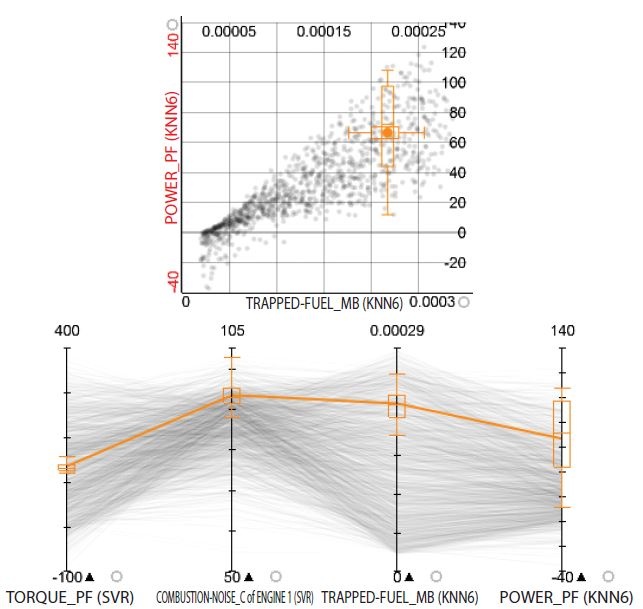
\includegraphics[width=0.6\textwidth]{figures/visualisation.jpg}
\caption{Representation of uncertainties in a scatter plot and parallel coordinates plot. The probability density function is visualised as a box-plot around a selected solution. Reproduced from~\cite{Berger2011uncertainty}.}
\label{fig:visualisation}
%% label for entire figure
\end{figure}

\section{Conclusion}
\label{sec:conclusion}
\subsection{Meeting WP1 requirements}
The framework presented in this document provides solutions to the requirements identified as crucial for this work-package. A summary of the framework's ability to meet the ``must have" and ``should have" requirements, defined in the previous milestone, is given in Tables~\ref{tab:requirements} and~\ref{tab:should have requirements}, respectively. The requirements are referred to by the numbering in WP1 M3 document. Non-methodological requirements such as user interface are not included in this summary.

\begin{table}
\caption{Work package 1 ``must have" requirements addressed by the framework}
\begin{tabularx}{\textwidth}{lccX} \toprule
{\bf Req.}	& {\bf Covered}	& {\bf Section}							& \multicolumn{1}{c}{\bf Comments}	\\ \midrule
4.a			&  \cmark 		& \ref{subsec:Types of Variables}		& 									\\
5.a			&  \cmark 		& \ref{subsubsec:uncertain inputs}		& 									\\
5.b			&  \cmark		& \ref{subsec:Shared Decision Variables}& 									\\
6.a			&  \cmark		& \ref{subsec:preference}				& 									\\
6.b--c		&  \cmark		& \ref{subsec:constraints}				& 									\\
6.e			&  \xmark		& 										& The current preference scheme does not translate attributes ranking into targets / region of interest\\
7.a			&  \cmark		& \ref{sec:Robustness Indicators}		& 									\\
7.b			&  \cmark		& \ref{subsec:validation}				& 						 			\\
8.f			&  \cmark		& \ref{subsec:model fidelity}			& 						 			\\
9.a			&  \cmark		& \ref{subsubsec:simple uncertainty quantification},\ref{subsubsec:mixed complexity functions},\ref{subsec:convergence}	& \\
10.d		&  \cmark		& \ref{subsec:log}						& 									\\
11.a		&  \cmark		& \ref{subsec:log}						& 									\\
12--14,18.a &  \cmark		& \ref{subsec:Visualisation}			& 									\\
15			&  \cmark		& \ref{subsec:convergence}				& 									\\
18.b		&  \cmark		& \ref{subsec:Shared Decision Variables}& 									\\
\bottomrule
\end{tabularx}
\label{tab:requirements}
\end{table}

\begin{table}
\caption{Recommendations for WP1 ``should have" requirements}
\begin{tabularx}{\textwidth}{lccX} \toprule
{\bf Req.}	& {\bf Covered}	& {\bf Section}						& \multicolumn{1}{c}{\bf Comments}	\\ \midrule
5.a.$iii$	&  \cmark 		& \ref{subsec:Types of Variables}	& 									\\
5.c			&  \cmark 		& \ref{subsec:model fidelity}		& 									\\
6.d			&  \cmark 		& \ref{subsec:preference}			& 									\\
6.j			&  \xmark 		& 									& This is addressed in WP2 and WP3	\\
6.k			&  \cmark 		& \ref{subsec:constraints}			& 									\\
8.g			&  \cmark 		& \ref{subsec:model fidelity}		& 									\\
9.d			&  \cmark 		& \ref{subsubsec:simple uncertainty quantification}	& 					\\
9.e			&  \xmark 		& 									& Customising the algorithm has a low priority at this stage \\
9.g			&  \cmark 		& 									& The algorithm is set with default parameters \\
11.b		&  \cmark		& \ref{subsec:log}					& 									\\
13.b, 16	&  \xmark		& 									& It would be beneficial to include these features if the project's time-scale allows \\
\bottomrule
\end{tabularx}
\label{tab:should have requirements}
\end{table}

\subsection{Framework limitations and risks}
This section summarises the assumptions made within the framework described in this document, and the risks associated with these assumptions.
\begin{itemize}
	\item \emph{The landscape is well behaved (i.e., smooth, continuous).} The uncertainty distributions are approximated according to available information for other candidate solutions. The underlying assumption for approximating in this way is that similar solutions have similar performance. If the functions are highly ragged and discontinuous, the surrogate models cannot accurately predict their behaviour.
	\item \emph{The dimensionality is small to medium.} The search is conducted on a surrogate model fitted to the existing evaluated solutions. The DACE model used in this framework typically produces good estimates for problems with up to 20 design variables.
	\item \emph{The problem formulation is appropriately elicited.} The outcomes from any use of the framework can only be as good as the information provided to it. Methodologies for robustly eliciting the problem formulation lie outside the scope of the project.
\end{itemize}

\subsection{Next steps in WP1}
Most of the methods described in this document have now been implemented in Tigon as part of WP1. Some development work remains to produce a working version. The next stages to verify the methodology are as follow:
\begin{itemize}
	\item Study the behaviour of sParEGO with a set of controllable stochastic multiobjective problems. A tool for constructing this sort of benchmark problems was created for this purpose. By controlling the difficulty of the multiobjective problem and the characteristics of the uncertainties, both the algorithm's performance and the effects of decision facilitator's choices can be examined.
	\item Complete the formulation of a pseudo case study for a robust design optimization problem, demonstrating all complexities addressed by this document. The problem will be implemented in software that can be interfaced to Liger (e.g. Matlab) and documented in the M5 report.
	\item Demonstrate the use of the framework on the pseudo case study problem, and document these findings in the M6 report. By this stage, the user interface and visualisation tools will have been implemented in Liger.
	\item Write the M8 report that concludes WP1. The report will highlight the strengths of the framework and its potential added value over existing practice conducted in JLR. Recommendations for further development towards a higher technology-readiness-level will be provided.
\end{itemize}


\bibliographystyle{IEEEtran}
\bibliography{WP1M4References}

\end{document}